\documentclass[xcolor=dvipsnames]{beamer}
\usepackage{amsmath}
\usepackage{amssymb}
\usepackage[english]{babel}
\usepackage[latin1]{inputenc}
\usepackage{times}
\usepackage[T1]{fontenc}
\usepackage{graphicx}
\usepackage[absolute, overlay]{textpos}
\usepackage{tikz}
\usepackage{multimedia}
\usepackage{soul}
\usepackage{hyperref}
\usepackage{wasysym}
\usepackage{cancel}
\def\urltilda{\kern -.15em\lower .7ex\hbox{\~{}}\kern .04em}
\def\deg{^{\circ}}

\setlength{\TPHorizModule}{0.01\textwidth}
\setlength{\TPVertModule}{\TPHorizModule}

\definecolor{darkyellow}{rgb}{1,0.75,0}
\definecolor{black}{rgb}{0,0,0}
\definecolor{orange}{rgb}{0.9, 0.5, 0.0}

\mode<presentation>
{
  \usetheme{Warsaw}
  \usecolortheme[named=darkyellow]{structure}	
  \setbeamercovered{transparent}
  \setbeamercolor{item}{fg=black}
}

%\beamerdefaultoverlayspecification{<+->}

\newcommand{\vect}[1]{\boldsymbol{#1}}
\newcommand{\params}{\Xi}
\newcommand{\Eobsi}{E'_i}
\newcommand{\phiobsi}{\phi'_i}
\newcommand{\Etruei}{E_i}
\newcommand{\phitruei}{\phi_{i}}
\newcommand{\Eobsij}{E'_{ij}}
\newcommand{\phiobsij}{\phi'_{ij}}
\newcommand{\Etrueij}{E_{ij}}
\newcommand{\phitrueij}{\phi_{ij}}
\newcommand{\obs}{\mathrm{obs}}
\newcommand{\true}{\mathrm{true}}
\newcommand{\Like}{\mathcal{L}}
\newcommand{\ntot}{{n_\mathrm{tot}}}
\newcommand{\ntotj}{{n_{\mathrm{tot},j}}}
\newcommand{\diff}{\mathrm{d}}
\newcommand{\cblue}[1]{{\color[rgb]{0.1, 0.0, 0.6} #1}}
\newcommand{\cgreen}[1]{{\color[rgb]{0.0, 0.6, 0.1} #1}}
\newcommand{\corange}[1]{{\color[rgb]{0.9, 0.5, 0.0} #1}}
\newcommand{\cbluewhen}[2]{{\color#2[rgb]{0.1, 0.0, 0.6} #1}}
\newcommand{\cgreenwhen}[2]{{\color#2[rgb]{0.0, 0.6, 0.1} #1}}
\newcommand{\corangewhen}[2]{\vspace{-1.4mm}{\color#2[rgb]{0.9, 0.3, 0.0} #1}}
\newcommand{\vrel}{v_{\mathrm{rel}}}
\newcommand{\mn}{m_{\rm nuc}}
\newcommand{\mx}{m_\chi}
\newcommand{\nc}{\newcommand}
\nc{\x}{{\bf x }}
\nc{\kk}{{\bf k }}
\nc{\f}{{\bf f }}
\nc{\e}{{\bf e }}
\nc{\gag}{g_{a \gamma}}
\nc{\ud}{\mathrm{d}}
\nc{\igev}{GeV$^{-1}$}
\nc{\ssi}{\sigma_{\mathrm{SI}}}
\nc{\ssd}{\sigma_{\mathrm{SD}}}
\nc{\tq}{\tilde \q}
\nc{\qmin}{q_{\mathrm{min}}}
\nc{\qmax}{q_{\mathrm{max}}}
\nc{\dmin}{\delta_{\mathrm{min}}}
\nc{\dmax}{\delta_{\mathrm{max}}}
\nc{\ie}{i.e.\xspace}
\nc{\del}{\partial}
\nc{\Cin}{C_{\mathrm{in}}}
\nc{\Cout}{C_{\mathrm{out}}}
\nc{\shat}{\hat \sigma}
\nc{\ket}[1]{| #1 \rangle}
\nc{\bra}[1]{\langle #1 |}
\nc{\braket}[2]{\langle #1 | #2 \rangle}
\nc{\speclarrow}{$\boldsymbol{\rightarrow}$\ }
\nc{\bi}{\begin{itemize}}
\nc{\ei}{\end{itemize}}
\nc{\bfr}[1]{\begin{frame}\frametitle{#1}}

\setbeamercolor{section in toc}{fg=darkgray}

\AtBeginSection[]
{
  \begin{frame}<beamer>
    \frametitle{Outline}
  \begin{columns}[t]
	\column{0.8\textwidth}
	\tableofcontents[sections={1},currentsection]
        \vspace{3mm}
	\tableofcontents[sections={2},currentsection]
        \vspace{3mm}
	\tableofcontents[sections={3},currentsection]
  \end{columns}	
  \end{frame}
}

\setbeamertemplate{subsection in head/foot shaded}
{\textcolor{structure!80!black}{\insertsubsectionhead}}
\setbeamertemplate{subsection in head/foot}{\textcolor{black}\insertsubsectionhead}

\title[{\color[rgb]{0, 0, 0}A preview of GAMBIT}]{\textcolor{black}{A preview of GAMBIT}}
\author[Pat Scott -- April 2015 -- IFT Madrid]{Pat Scott}
\institute{\small{Imperial College London}}
\date[April 2015]{\small \centering on behalf of the GAMBIT Collaboration \\\cblue{\href{http://gambit.hepforge.org}{http://gambit.hepforge.org}}}
\subject{Talks}
\pgfdeclareimage[height=0.7cm]{university-logo}{Logo2}
\logo{\pgfuseimage{university-logo}}

\begin{document}

\maketitle

\begin{frame}
  \frametitle{Let's begin with dessert.}

GAMBIT: The \alert{G}lobal \alert{A}nd \alert{M}odular \alert{B}SM \alert{I}nference \alert{T}ool
\vspace{2mm}

  \visible<2->
  {
    \begin{exampleblock}{So what \textit{\textbf{is}} GAMBIT?}
      \visible<3->
      {
        3 things:
        \visible<4->
        {
          \bi
            \item A collaboration of about thirty theorists and experimentalists
            \visible<5->{
            \item A new public global fitting code
            \visible<6->{
            \item A program of physics analyses that we're carrying out using the code}}
          \ei
        }
      }
    \end{exampleblock}
  }
  
  \visible<7->{
  \vspace{2mm}
  First physics results and code release in a few months\\
  (i.e.\ late summer \alert{this year})
  }
  
\end{frame}

\begin{frame}
  \frametitle{Outline}
  \begin{columns}[t]
	\column{0.8\textwidth}
	\tableofcontents[sections={1}]
        \vspace{3mm}
	\tableofcontents[sections={2}]
        \vspace{3mm}
	\tableofcontents[sections={3}]
  \end{columns}	
\end{frame}

\section{The problem}

\begin{frame}
\frametitle{Combining searches {\rm I}}

  \begin{exampleblock}{Question}
  How do we know which models are in and which are out?
  \end{exampleblock} 

  \visible<2->{
  \begin{block}{Answer}
  Combine the results from different searches
  \end{block}

\begin{columns}[c]
\column{0.5\textwidth}
\footnotesize
\begin{itemize}
\item Simplest method: take different exclusions, overplot them, conclude things are ``allowed'' or ``excluded''
\item Simplest BSM example: the scalar singlet model
\vspace{1cm}
\end{itemize}
\column{0.45\textwidth}
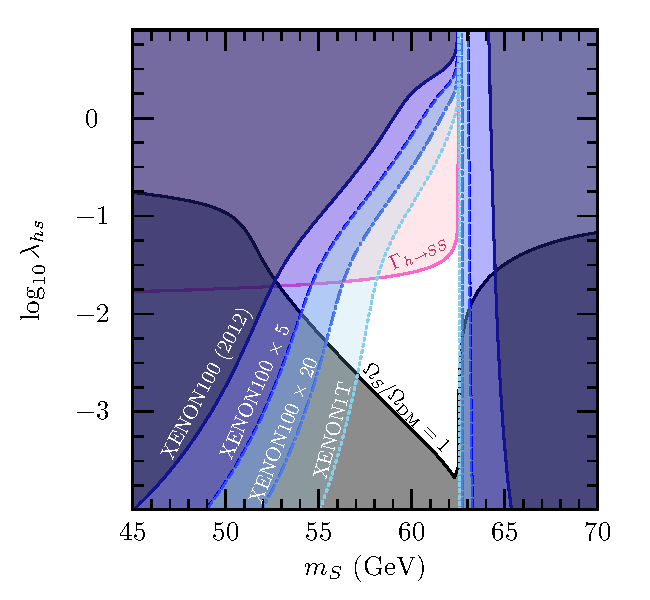
\includegraphics[width=\textwidth]{Fig6a}
\column{0.10\textwidth}
\end{columns}
}

  \begin{textblock}{80}(10,75)
  \visible<2->{\tiny(Cline, Kainulainen, PS \& Weniger, \textit{PRD}, 1306.4710)}
  \end{textblock}

\end{frame}


\begin{frame}
\frametitle{Combining searches {\rm II}}

That's all well and good if there are only 2 parameters and few searches\ldots\vspace{3mm}

  \begin{exampleblock}{Question}
  What if there are many different \alert{constraints}?
  \end{exampleblock} 

  \visible<2->
  {
    \begin{columns}[c]
    \column{0.4\textwidth}
      \begin{block}{Answer}
        Combine constraints in a statistically valid way \\$\rightarrow$ composite likelihood
      \end{block}\vspace{10mm}
    \column{0.45\textwidth}
      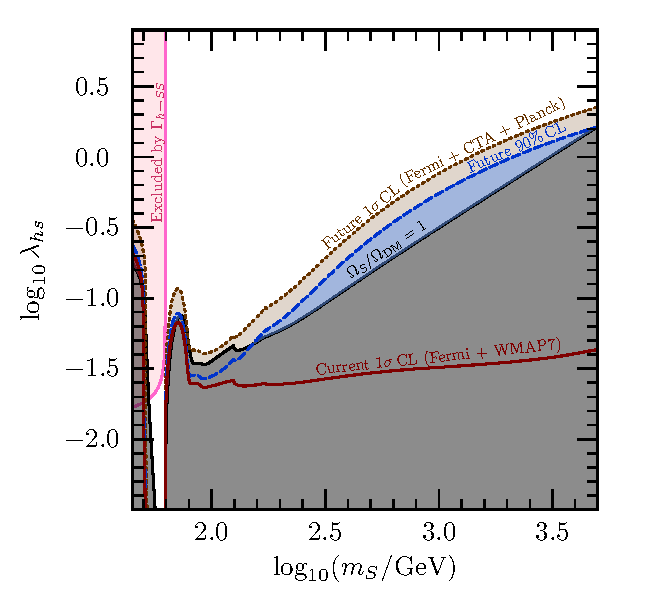
\includegraphics[width=\textwidth]{Fig3b}
    \end{columns}  
  }

  \begin{textblock}{80}(20,75)
  \visible<2->{\tiny(Cline, Kainulainen, PS \& Weniger, \textit{PRD}, 1306.4710)}
  \end{textblock}

\end{frame}


\begin{frame}
\frametitle{Combining searches {\rm III}}

That's all well and good if there are only 2 parameters and few searches\ldots\vspace{3mm}

  \begin{exampleblock}{Question}
  What if there are many \alert{parameters}?
  \end{exampleblock}

\visible<2->{
\begin{block}{Answer}
Need to 
\begin{itemize}
\item scan the parameter space (smart numerics)
\item interpret the combined results (Bayesian / frequentist)
\item project down to parameter planes of interest (marginalise / profile)
\end{itemize}
$\rightarrow$ \alert{global fits}
\end{block}}\vspace{3mm}

\end{frame}



\begin{frame}
\frametitle{Beyond-the-Standard-Model Scanning}

  \alert{Goals:} 
  \begin{enumerate} 
    \item Given multiple theories, determine which fit the data better, and quantify how much better \visible<2->{\cblue{$\implies$ model comparison}}
    \item Given a particular theory, determine which parameter combinations fit all experiments, and how well \visible<2->{\\\hspace{5.15cm}\cblue{$\implies$ parameter estimation}}
  \end{enumerate} 
  \vspace{4mm}

\visible<3>{
Why simple IN/OUT analyses are not enough\ldots
\vspace{2mm}
\small
\begin{itemize}
\item Only partial goodness of fit, no measure of convergence, no idea how to generalise to regions or whole space.
\item Frequency/density of models in IN/OUT scans is \\\alert{not} proportional to probability $\implies$ no statistical meaning.
\item $\rightarrow$ statements about a theory's general ability to do one thing or another, based on such scans, are statistically invalid
\end{itemize}
\vspace{2mm}
}

\end{frame}



\section{Future challenges}

\begin{frame}
\frametitle{The LHC likelihood monster}

\begin{textblock}{30}(80.6,10.2)
    
\includegraphics[width=\linewidth]{LHCmonster}
\end{textblock}

\visible<1->{
\begin{exampleblock}{Time per point:}
$\mathcal{O}(minute)$ in \alert{best} cases
\end{exampleblock}
}

\visible<2->{
\begin{exampleblock}{Time per point for global fits to converge:}
$\mathcal{O}(seconds)$ in \alert{worst} cases
\end{exampleblock}
}

\visible<3->{
\begin{exampleblock}{Challenge:}
About 2 orders of magnitude too slow to actually include LHC data in global fits properly
\end{exampleblock}
}

\visible<4->{
\vspace{2mm}
\alert{$\rightarrow$ More in Martin's presentation}
}

\end{frame}

\begin{frame}
\frametitle{Doing genuinely `model-independent' DM pheno}

\visible<1->{
\begin{exampleblock}{All experimental limits in terms of simplified models: effective WIMP, one annihilation channel, etc}
$\implies$ need something to apply limits to arbitrary DD couplings and ID decay/annihilation branching fractions\\
$\implies$ must include accurate treatment of experimental effects
\end{exampleblock}
}

\visible<2->{
\begin{exampleblock}{Impacts of new unstable particles (e.g. extra Higgs) are hard}
$\implies$ need to simulate decays `on the fly'
\end{exampleblock}
}

\visible<3->{
\begin{exampleblock}{Calculating relic densities for general models also challenging}
$\implies$ want to feed in partial annihilation rates, co-annihilations, resonances, etc (not only set up model in LanHEP)
\end{exampleblock}
}

\visible<4->{
\vspace{2mm}
\alert{$\rightarrow$ nulike, gamlike, DDcalc, cascade sim $\rightarrow$ Christoph's talk}
}

\end{frame}


\begin{frame}
\frametitle{Parameter space $\rightarrow$ Theory space}

\alert{CMSSM, MSSM, Simplified Models $\ne$ BSM}
\vspace{3mm}

Want to do model comparison to actually work out which theory is the best\ldots
\vspace{3mm}

\begin{exampleblock}{Challenge:}
How do I easily adapt a global fit to different BSM theories?
\end{exampleblock}

\visible<2>{
Somehow, we must recast things quickly to a new theory 
\begin{itemize}
\item data
\item likelihood functions
\item scanning code `housekeeping'
\item even predictions
\end{itemize}
$\implies$ a new, very abstract global fitting framework
}

\end{frame}

\begin{frame}
\frametitle{Hitting the wall}

Issues with current global fit codes:
\begin{itemize}
\item Strongly wedded to a few theories (e.g. constrained MSSM / mSUGRA)
\item Strongly wedded to a few theory calculators
\item All datasets and observables basically hardcoded
\item Rough or non-existent treatment of most experiments (astroparticle + collider especially)
\item Sub-optimal statistical methods / search algorithms
\item $\implies$ \textit{already hitting the wall on theories, data \& computational methods}
\end{itemize}

\end{frame}

\section{Future solutions}

\begin{frame}
\frametitle{\textbf{GAMBIT}: a \textit{second-generation} global fit code}

GAMBIT: \alert{G}lobal \alert{A}nd \alert{M}odular \alert{B}SM \alert{I}nference \alert{T}ool
\vspace{5mm}

Overriding principles of GAMBIT: flexibility and modularity
\begin{itemize}
\item General enough to allow fast definition of new datasets and theoretical models
\item Plug and play scanning, physics and likelihood packages
\item Extensive model database -- not just small modifications to constrained MSSM (NUHM, etc), and not just SUSY!
\item Extensive observable/data libraries (likelihood modules)
\item Many statistical options -- Bayesian/frequentist, likelihood definitions, scanning algorithms
\item A smart and \textit{fast} LHC likelihood calculator
\item Massively parallel
\item Full open-source code release
\end{itemize}

\end{frame}


\begin{frame}
\frametitle{The GAMBIT Collaboration}

26 Members, 15 institutions, 9 countries \\
8 Experiments, 4 major theory codes \vspace{2mm}

\scriptsize
\begin{columns}
\column{0.7\textwidth}
\begin{tabular}{l l}
\textbf{Fermi-LAT} &  J.\ Conrad, J.\ Edsj\"o, G.\ Martinez\\
                   & \alert<2>{P.\ Scott}\vspace{0.5mm}\\
\textbf{ATLAS} &  A.\ Buckley, P.\ Jackson, C.\ Rogan,\\
               & A.\ Saavedra, \alert<2>{M.\ White}\vspace{0.5mm}\\
\textbf{CTA} &  C. Bal\'azs, T.\ Bringmann, \\
             & J.\ Conrad, \alert<2>{M.\ White}\vspace{0.5mm}\\
\textbf{HESS} &  J.\ Conrad \vspace{0.5mm}\\
\textbf{LHCb} &  M.\ Chrz\c{a}szcz, N.\ Serra\vspace{0.5mm}\\
\textbf{IceCube} &  J.\ Edsj\"o, C.\ Savage, \alert<2>{P.\ Scott}\vspace{0.5mm}\\
\textbf{AMS-02} &  A.\ Putze\vspace{0.5mm}\\
\textbf{CDMS, DM-ICE} &  L. Hsu\vspace{0.5mm}\\
\textbf{XENON/DARWIN} &  J.\ Conrad\vspace{0.5mm}\\
\textbf{Theory} &  P.\ Athron, C. Bal\'azs, T.\ Bringmann, \\
                & \alert<2>{J.\ Cornell}, L.\ Dal, J.\ Edsj\"o, \alert<2>{B.\ Farmer},\\
                & A.\ Krislock, A.\ Kvellestad, M.\ Pato, \\
                & F.\ Mahmoudi, A.\ Raklev, C.\ Savage,\\
                & \alert<2>{P.\ Scott}, \alert<2>{C.\ Weniger}, \alert<2>{M.\ White} \\	
\end{tabular}
\column{0.4\textwidth}
\end{columns}

\begin{textblock}{45}(73,13)
  
\includegraphics[width=\linewidth]{Logo2full}\\	
  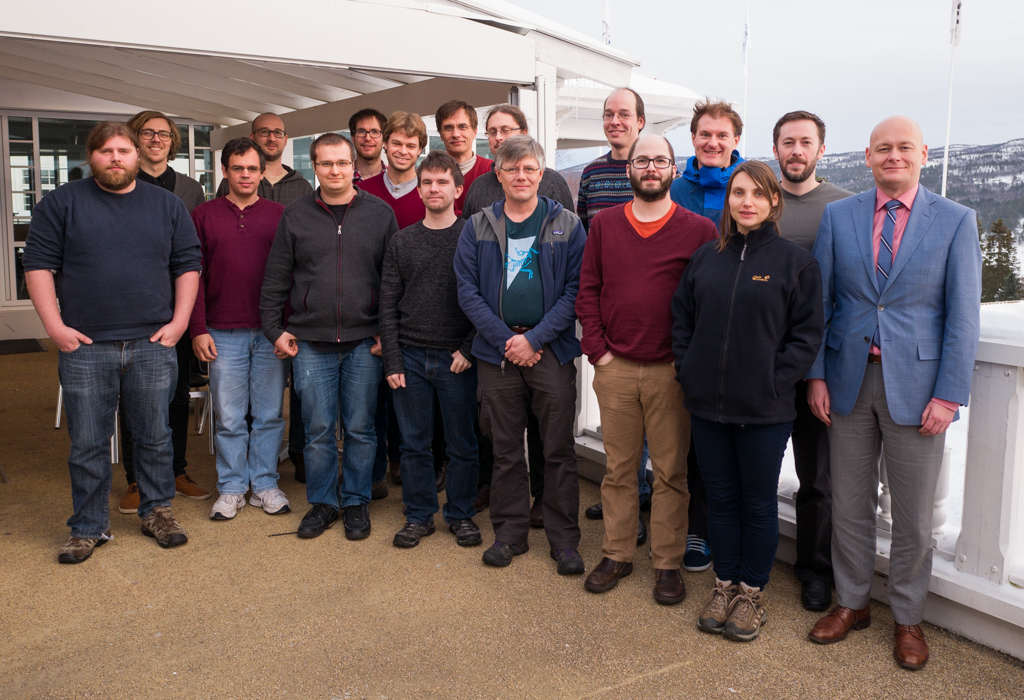
\includegraphics[width=\linewidth]{GroupPhoto}
\end{textblock}

\end{frame}

\begin{frame}
\frametitle{Modules}

Physics Modules
\begin{itemize}
\corange{\item ColliderBit} (Martin's talk)
\corange{\item DarkBit} (Christoph's talk)
\corange{\item FlavBit} -- flavour physics inc. $g-2$, $b\rightarrow s\gamma$, $B$ decays (new channels, theory uncerts, LHCb likelihoods)
\corange{\item SpecBit} -- generic BSM spectrum object, providing RGE running, masses, mixings, etc via interchangeable interfaces to different RGE codes
\corange{\item DecayBit} -- decay widths for all relevant SM \& BSM particles
\corange{\item EWPOBit} -- precision tests (mostly by interface to FeynHiggs, alt. SUSY-POPE)
\end{itemize}

+\corange{ScannerBit}: manages statistics, parameter sampling and optimisation algorithms

\end{frame}


\begin{frame}
\frametitle{Backends: mix and match}

\bi
\item GAMBIT modules consist of a number of standalone \textbf{module functions}
\item Module functions can depend on each other, or they can require specific functions from \textbf{backends}
\item Backends are external code libraries (DarkSUSY, FeynHiggs, etc) that include different functions 
\item GAMBIT automates and abstracts the interfaces to backends $\rightarrow$ backend functions are tagged according to \alert{what they calculate}
\item $\rightarrow$ with appropriate module design, \alert{different backends and their functions can be used interchangeably}
\item GAMBIT dynamically adapts to use whichever backends are actually present on a user's system (+ provides details of wtf it did of course)
\ei

\only<2>{
\begin{textblock}{110}(10,30)
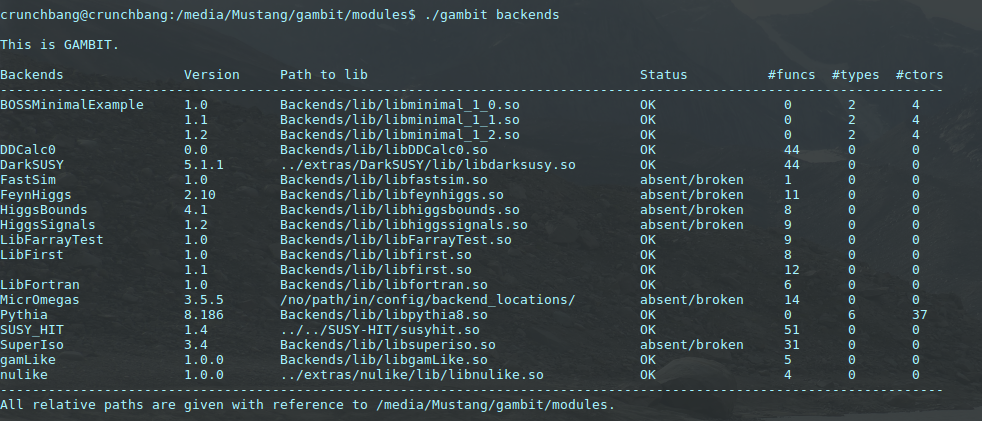
\includegraphics[width=\textwidth]{backendshot}
\end{textblock}
}

\end{frame}

\begin{frame}
\frametitle{GAMBIT: a toy example}
\centering
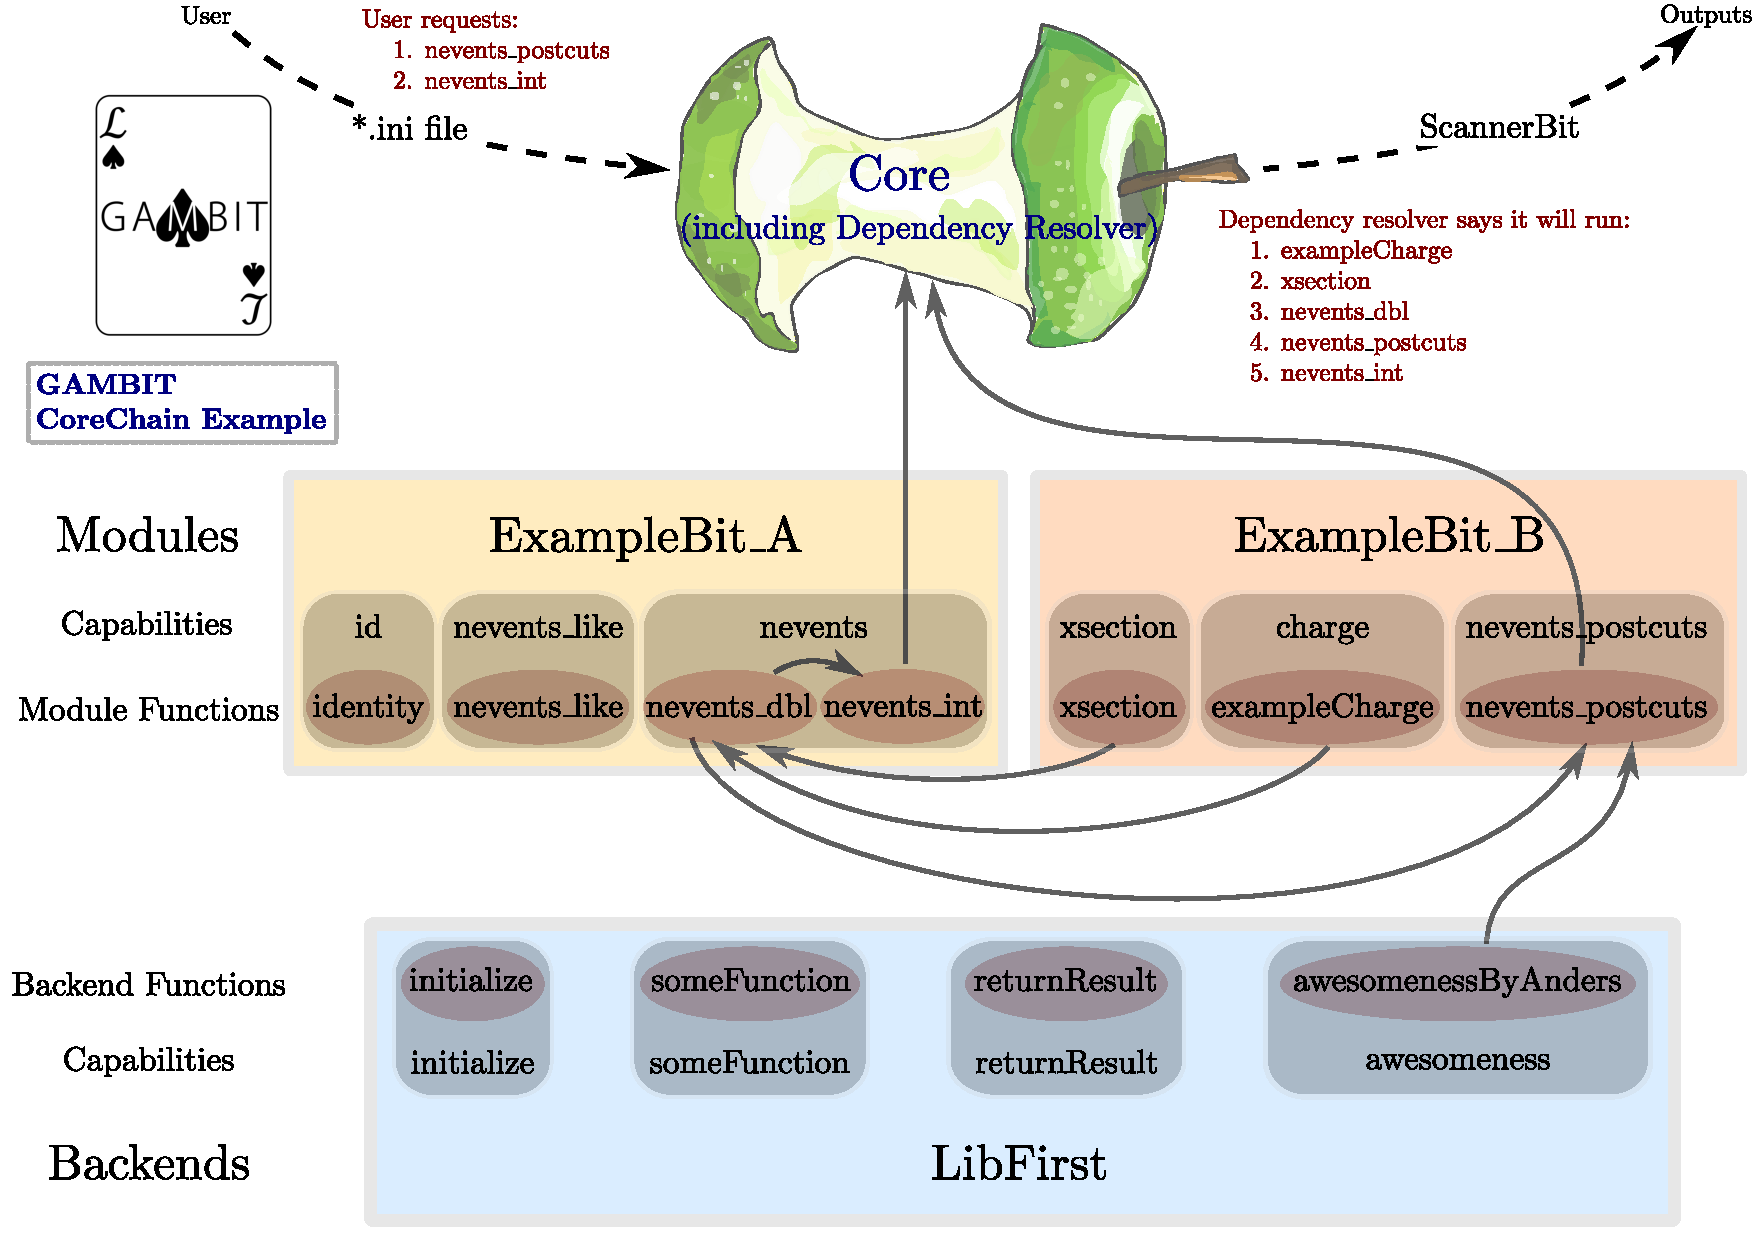
\includegraphics[width=0.9\textwidth]{coreChainDiagram_example_wlogo}	
\end{frame}

\begin{frame}
\frametitle{Dependency Resolution}

\uncover<1>
{
  \bi
    \item Module functions and backend functions get arranged into a \textbf{dependency tree}
    \item Starting with requested observables and likelihoods, fills each dependency and backend requirement
    \item Obeys rules at each step: allowed models, allowed backends, constraints from input file, etc
    \item $\rightarrow$ tree constitutes a directed acyclic graph
    \item $\rightarrow$ GAMBIT uses graph-theoretic methods to `solve' the graph to determine function evaluation order
  \ei
}

\visible<1>
{
  \includegraphics[width=\textwidth]{GAMBIT_active_functor_graph}
}

\only<2>{
\begin{textblock}{73}(45,17)
\includegraphics[width=\textwidth, trim = 0 0 8000 0, clip=true]{GAMBIT_active_functor_graph}
\end{textblock}
}

\end{frame}


\begin{frame}
\frametitle{Hierarchical Model Database}

\bi
  \item Models are defined by their parameters and relations to each other
  \item Models can inherit from \textbf{parent models}
  \item Points in child models can be \textbf{automatically translated} to ancestor models
  \item \textbf{Friend models} also allowed (cross-family translation)
  \item Model dependence of every module/backend function is tracked $\implies$ \alert{maximum safety, maximum reuse}
\ei

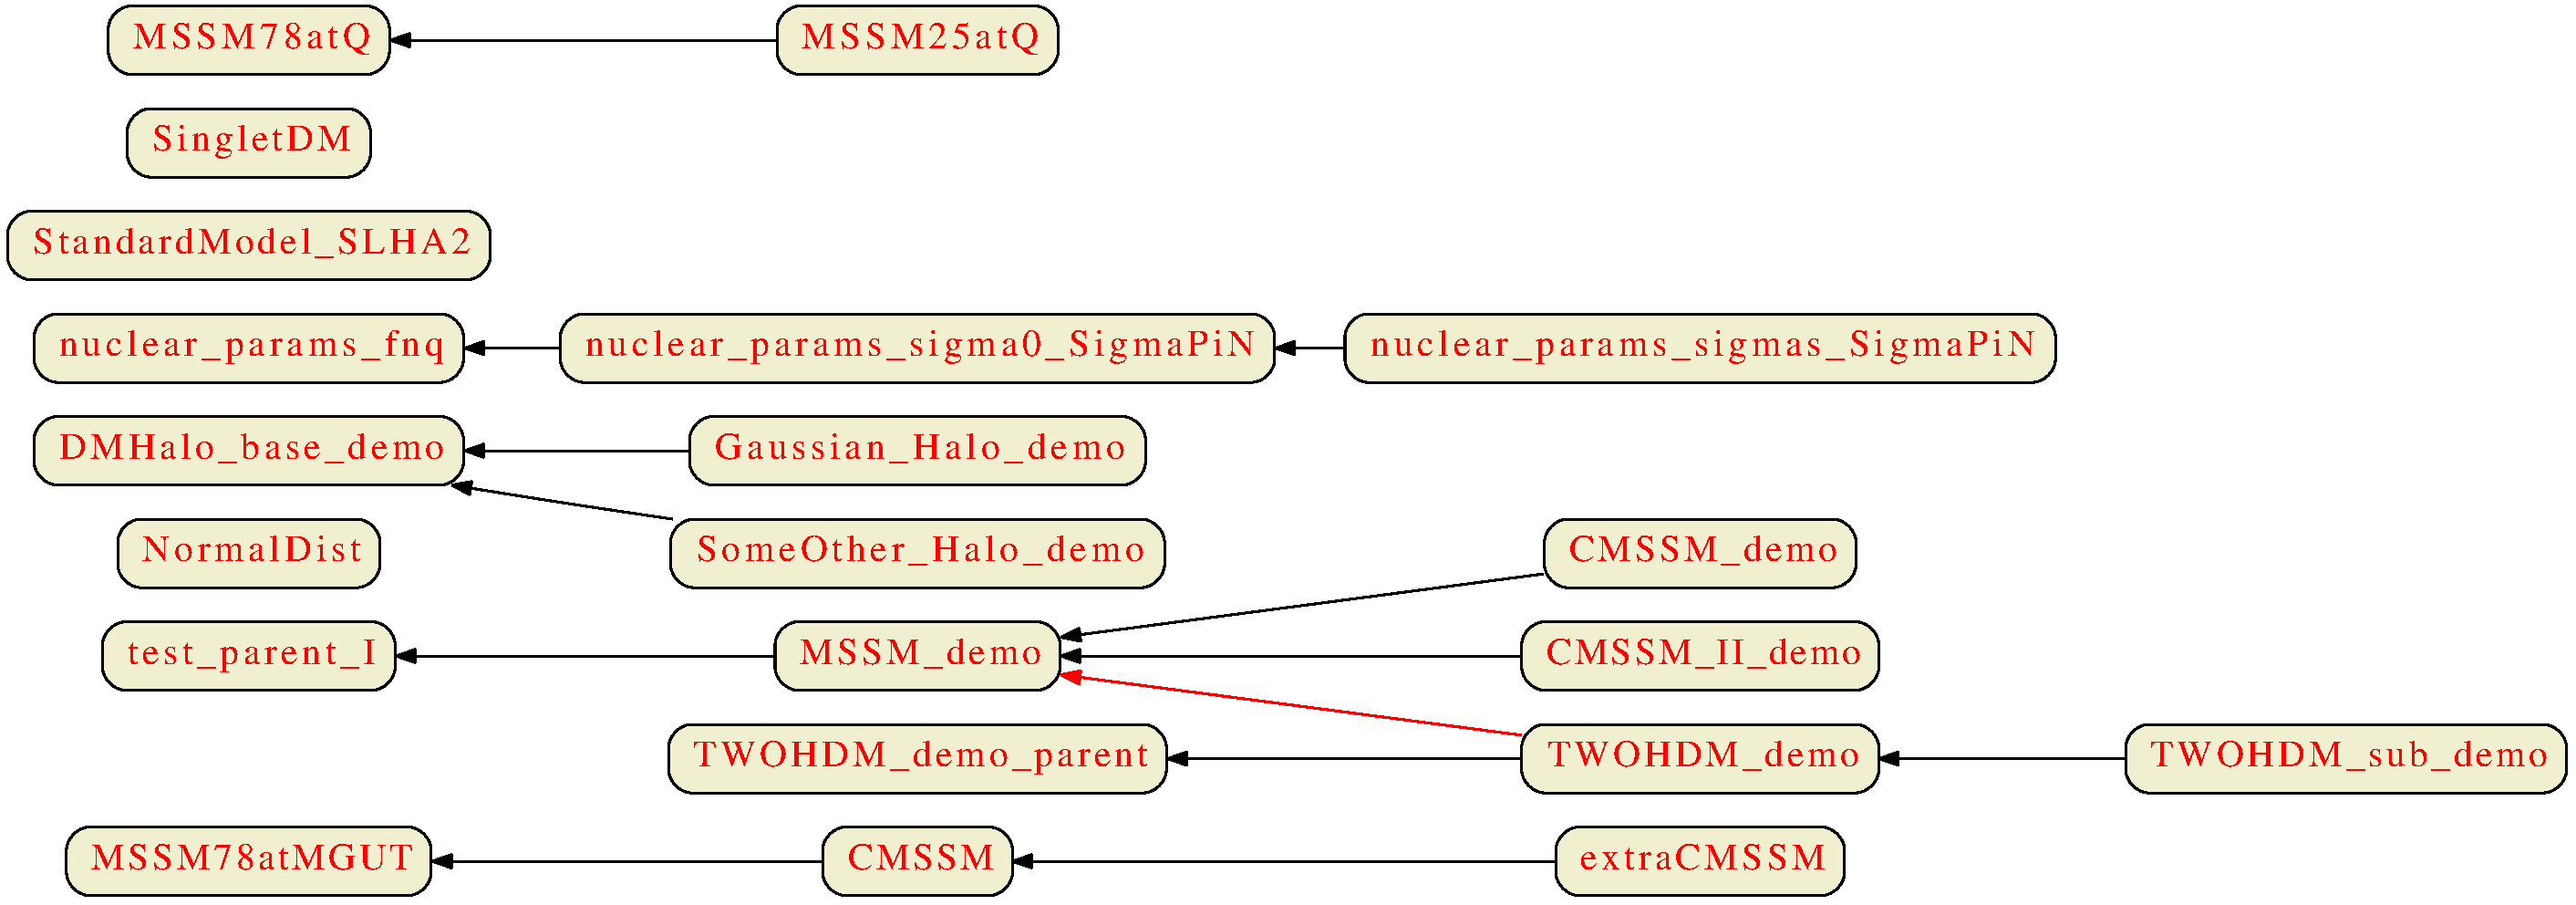
\includegraphics[width=0.8\textwidth]{GAMBIT_model_hierarchy}

\end{frame}

\begin{frame}
\frametitle{Interface: yaml file}

Basic interface for a scan is a YAML initialisation file
\begin{columns}
\column{0.6\linewidth}
\bi
\item[-] \alert<2>{specify parameters, ranges, priors}
\item[-] \alert<3>{select likelihood components}
\item[-] \alert<3>{select other observables to calculate}
\item[-] \alert<4>{define generic rules for how to fill dependencies}
\item[-] \alert<4>{define generic rules for options to be passed to module functions}
\item[-] \alert<5>{set global options (scanner, errors/warnings, logging behaviour, etc)}
\ei
\column{0.5\linewidth}
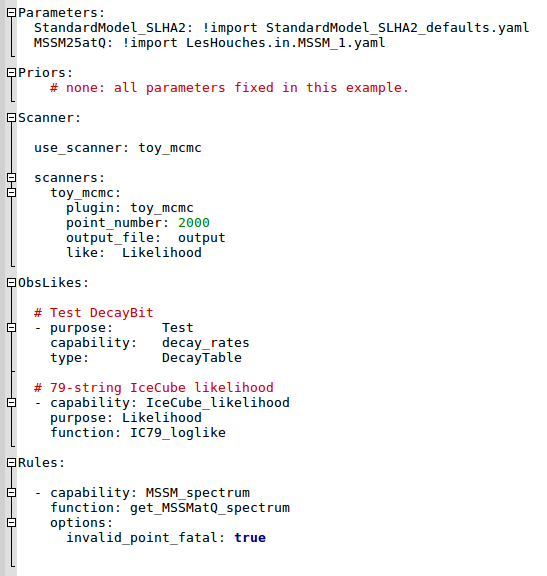
\includegraphics[width=1.2\textwidth]{yamlshot}
\end{columns}

\begin{textblock}{20}(55,20)
  \visible<2>
  {
    
\begin{tikzpicture}
      \draw[color=red,line width=0.07cm]
            (0,0) ellipse (3.0 and 0.8);
    \end{tikzpicture}
  }
\end{textblock}

\begin{textblock}{20}(55,49)
  \visible<3>
  {
    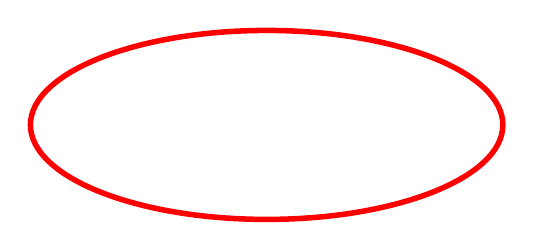
\begin{tikzpicture}
      \draw[color=red,line width=0.07cm]
            (0,0) ellipse (3.0 and 1.2);
    \end{tikzpicture}
  }
\end{textblock}

\begin{textblock}{20}(55,68)
  \visible<4>
  {
    
\begin{tikzpicture}
      \draw[color=red,line width=0.07cm]
            (0,0) ellipse (3.0 and 0.8);
    \end{tikzpicture}
  }
\end{textblock}

\begin{textblock}{20}(55,35)
  \visible<5>
  {
    
\begin{tikzpicture}
      \draw[color=red,line width=0.07cm]
            (0,0) ellipse (3.0 and 0.9);
    \end{tikzpicture}
  }
\end{textblock}

\end{frame}

\begin{frame}
\frametitle{Expansion: adding new functions}

Adding a new module function is easy:
\begin{enumerate}
\item Declare the function to GAMBIT in a module's \textbf{rollcall header}\bi
  \item Choose a capability
  \item Declare any \textbf{dependencies}
  \item Declare any \textbf{backend requirements}
  \item Declare any specific \textbf{allowed models}
  \item other more advanced declarations also available
\ei
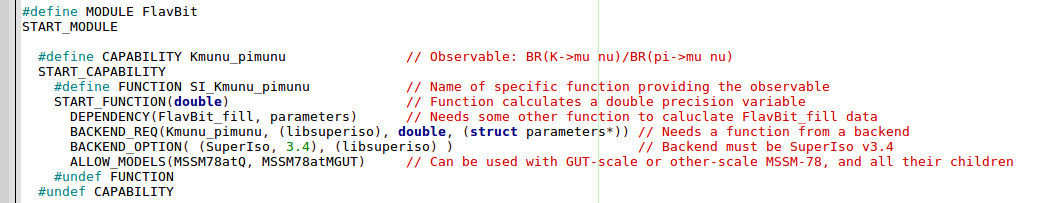
\includegraphics[width=\textwidth]{rollcallshot}
\item Write the function as a simple C$++$ function\\(one argument: the result)
\end{enumerate}


\end{frame}

\begin{frame}
\frametitle{Other nice technical features}
\bi
\item \textbf{Scanners}: MultiNest, Diver (diff.\ evolution), PIKAIA (genetic algorithms), GreAT (MCMC)
\item \textbf{Statistics}: Bayesian, Profile Likelihood, later full Neyman
\item Mixed-mode \textbf{MPI + openMP}, mostly automated
\item diskless generalisation of various Les Houches Accords
\item \textbf{BOSS}: dynamic loading of C++ classes from backends (!)
\item \textbf{all-in or module standalone} modes -- easily implemented from single cmake script
\item \textbf{automatic getters} for obtaining, configuring + compiling backends\footnote{if a backend breaks, won't compile and/or kills your dog, blame the\\\protect{\hspace{5mm}} authors (not us\ldots unless we \textbf{are} the authors\ldots)}  
\item \textbf{flexible output streams} (ASCII, databases, binary, \ldots)
\item more more more\ldots
\ei
\end{frame}


\begin{frame}
\frametitle{GAMBIT vs the rest -- in a nutshell}

\begin{columns}
\column{1.13\linewidth}

\tiny
\begin{tabular}{p{12mm}|p{36mm}|p{13mm}|p{13mm}|p{12mm}|p{12mm}}
\hline
Aspect & GAMBIT & MasterCode & SuperBayeS & Fittino & Rizzo et al. \\
\hline
\corangewhen{Design}{<2>} & \corangewhen{Modular, Adaptive}{<2>} & Monolithic & Monolithic & ($\sim$)Monolithic & Monolithic \\
\corangewhen{Statistics}{<3>} & \corangewhen{Frequentist, Bayesian}{<3>} & Frequentist & Freq./Bayes. & Frequentist & None \\
\corangewhen{Scanners}{<4>} & \corangewhen{Differential evolution, genetic algorithms, random forests, t-walk, t-nest, particle swarm, nested sampling, MCMC, gradient descent}{<4>} & Nested sampling, MCMC, grad.\ descent & Nested sampling, MCMC & MCMC & None (random) \\
\corangewhen{Theories}{<5>} & \corangewhen{(p)MSSM-25, CMSSM$\pm$$\epsilon$, GMSB, AMSB, gaugino mediation, E6MSSM, NMSSM, BMSSM, PQMSSM, effective operators, iDM, XDM, ADM, UED, Higgs portals/extended Higgs sectors}{<5>} & CMSSM$\pm$$\epsilon$ & (p)MSSM-15, CMSSM$\pm$$\epsilon$, mUED & CMSSM$\pm$$\epsilon$ & (p)MSSM-19 \\
\corangewhen{Astroparticle}{<6>} & \corangewhen{Event-level: IceCube, Fermi, LUX, XENON, CDMS, DM-ICE. Basic: $\Omega_{\rm DM}$, AMS-02, COUPP, KIMS, CRESST, CoGeNT, SIMPLE, PAMELA, Planck, HESS. Predictions: CTA, DARWIN, GAPS}{<6>}  & Basic: $\Omega_{\rm DM}$, LUX, XENON & Basic: $\Omega_{\rm DM}$, Fermi, IceCube, XENON & Basic: $\Omega_{\rm DM}$, Fermi, HESS, XENON & Event-level: Fermi.\newline Basic: $\Omega_{\rm DM}$, IceCube, CTA \\
\corangewhen{LHC}{<7>} & \corangewhen{ATLAS+CMS multi-analysis with neural net and fast detector simulation.  Higgs multi-channel with correlations and no SM assumptions. Full flavour inc. complete $B\to X_sll$ and $B\to K^*ll$ angular set.}{<7>} & ATLAS resim, HiggsSignals, basic flavour. & ATLAS direct sim, Higgs mass only, basic flavour. & ATLAS resim, HiggsSignals, basic flavour. & ATLAS+CMS\newline+Tevatron direct sim, basic flavour. \\
\corangewhen{SM, theory and related uncerts.}{<8>} & \corangewhen{$m_t$, $m_b$, $\alpha_{\rm s}$, $\alpha_{\rm EM}$, DM halo, hadronic matrix elements, detector responses, QCD+EW corrections (LHC+DM signal+BG), astro BGs, cosmic ray hadronisation, coalescence and p'gation.}{<8>} & $m_t$, $m_Z$, $\alpha_{\rm EM}$, hadronic matrix elements & $m_t$, $m_b$, $\alpha_{\rm s}$, $\alpha_{\rm EM}$, DM halo, hadronic matrix elems. & $m_t$ & None \\
\hline
\end{tabular}
\end{columns}

\end{frame}

\begin{frame}
\frametitle{Closing remarks}

\begin{itemize}
\item{Robust analysis of dark matter and BSM physics requires multi-messenger global fits}
\item{GAMBIT is coming:}\bi
\item[$\rightarrow$]{Global fits to many models for the first time}
\item[$\rightarrow$]{Better global fits to familiar ones}
\item[$\rightarrow$]{Highly modular, usable and extendable public code}
\item[$\rightarrow$]{Faster, more complete and more consistent theory explorations + experimental analysis prototyping} 
\ei
\end{itemize}

\end{frame}

\begin{frame}

\begin{textblock}{100}(0,-0.5)
  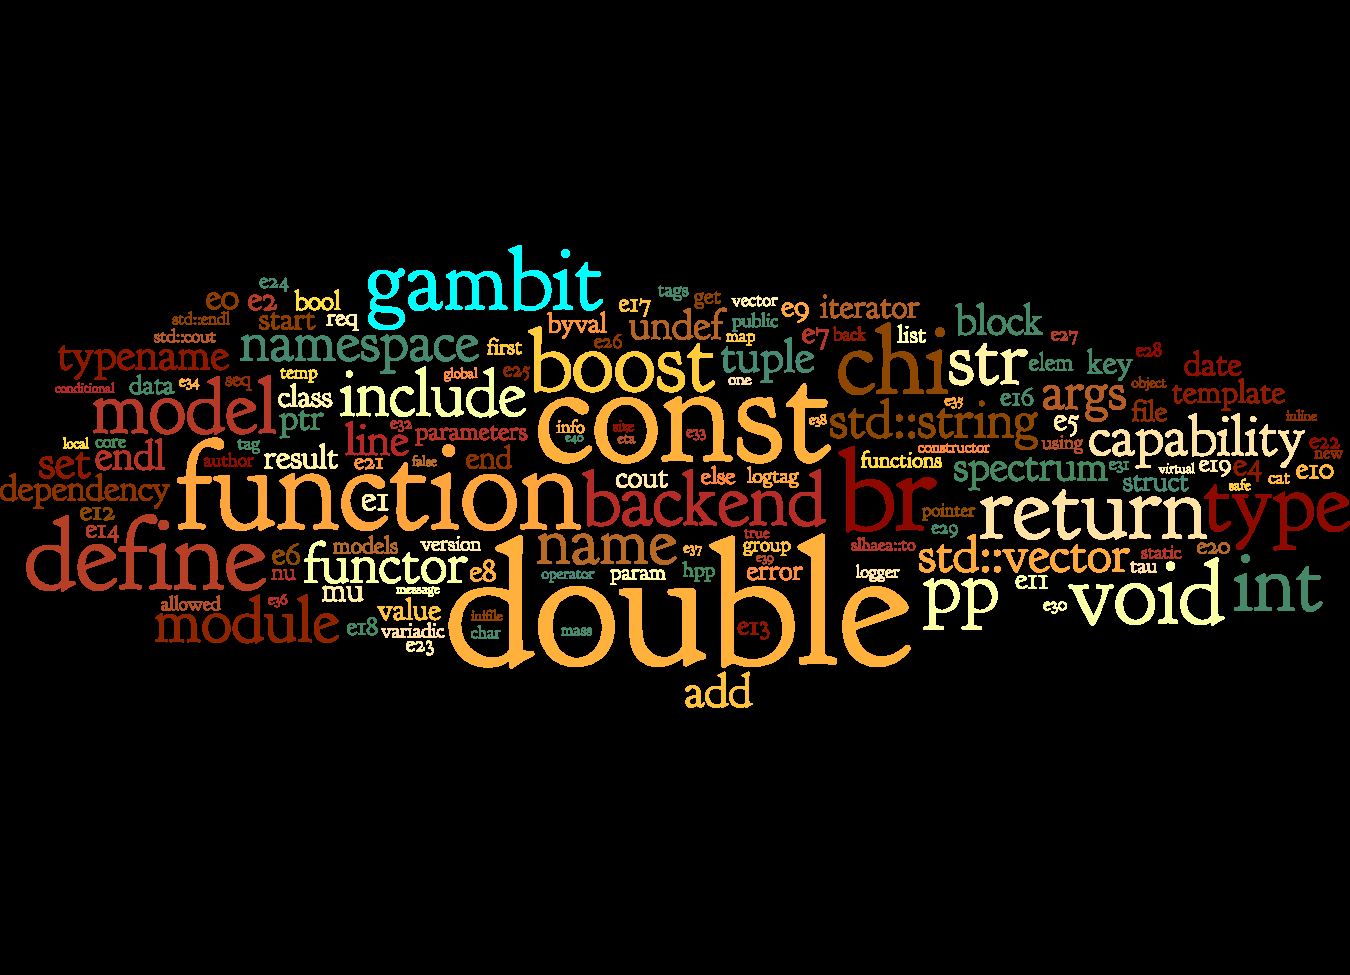
\includegraphics[width=1.19\linewidth]{GAMBIT_wordle}
\end{textblock}

\end{frame}




\end{document}

